\chapter{量子计算机与信息安全对密码学的影响}
\label{chap:2}

在本章量子计算机与信息安全对密码学的影响的部分,本作业尝试整理近来量子计算机的发展对信息安全领域的影响的研究与资讯,包括对密码学领域所带来的挑战与对策。当中所谓的量子计算与量子密码是根据量子力学与效应所发展的计算技术跟与相应发展的密码技术,其前者根据利用运行上千的量子位元跟量子算法的量子计算机的特性,在将来会直接挑战目前传统的资讯安全算法,从而导致目前广泛与大两使用的 RSA 密码手段被破解的可能,同时也使原本高强度的密码技术不如以往。
同时量子通信领域中的量子密钥分发技术也大大的改变了过往的模式,其于 1984 年由 Bennett 和 Brassard 两人所提出的第一个量子密钥分发协议,开始了量子密码学的研究,1994 年 Shor 运用量子 Fourier 变换的特性,去设计了第一个实用的量子算法,其原理则是在多项式时间内对大整数进行因子分解,另外于 1996 年 Grover提出了量子搜索算法,该法能够对无结构数据进行二次加速。此两个方法展现了量子计算的优越性,同时还对传统基于数学困难问题的密码学体制造成威胁。
本作业第一节为量子计算与通信的意义,第二节为量子力学的数学,第三节为量子计算的整理,第四节为量子算法的整理,第五节为量子通信与量子密码研究进展,最后进行结论。

%\begin{itemize}
%\item [-]IEEE 
%\end{itemize}

\section{发展量子计算与通信的意义}

对目前计算机发展影响深巨的在于电晶体与积体电路的发明,其相关发展带动目前消费者电子产品、智慧型手机、平板与个人电脑等不同嵌入式设备,在其市场的蓬勃发展,间接带动网际网路的发展。其中密码学演算法下的公钥密码演算法为基础,其保障人们可以在网路上安全的进行互动。

上述的发展皆从量子力学中发展而来,而所谓的量子力学则是研究微观尺度的量子物理理论,根据量子力学的原理,进而发展了半导体物理的理论,从而制造出电晶体与积体电路,同时量子通信等领域深入研究也导致新的改变。另外随着近年该领域的不断发展,也出现如量子时钟、量子成像、量子传感、量子计算与通信等具有巨大应用潜力的技术应用,而当中与资讯安全相关的为量子计算和量子通信。

\subsection{量子计算的部分}

根据摩尔定律,在成本不变的情况下,每隔 18 至 24 个月,在积体电路上可容纳的电晶体密度会增加一倍。虽然其定律在过往半世纪以来相当有效,但随着电晶体大小缩小到原子大小,半导体的会面对无法散热跟漏电的问题,导致无法运作。所以若想继续发展更大计算能力的计算机,则可能要另辟蹊径,当中使用量子算法的量子计算机很可能即为这当中的具有希望的方案之一,由此来满足人们对于此的需求。

此外另一个重点是量子计算机对资讯安全的影响在于,一旦通用型的量子计算机发展到可以处理的量 子 位元数目达到一定规模后,现有传统的密码学体制将会被量子的 Shor 演算法轻松地破解,当下现在网际网路上进行的通信和金融交易等活动的安全皆将会受到直接的挑战,其解决办法是将这些演算法更换为可以抵抗量子计算攻击的密码演算法。

\subsection{量子通信的部分}

量子通信技术领域中相对成熟的应用是量子密钥分发及其相关技术,而传统密码技术的一大困难是在于无法真正保证通信双方共享的密钥的不分是绝对安全,也因此经典的位元十分容易复制且不易被察觉,所以通信双方无法真正确认共享密钥是否已被恶意攻击者获取。而量子通信技术利用光子的量子特性,在传输量子信息的过程中,一旦受到窃听和破坏,必然会引入干扰 ,这样就可以通过物理的手段将攻击行为检测出来,保证信息传输的安全 ,从根本上解决点对点的密钥分发问题,确保点对点通信的安全。也因此量子密钥分发有时也被称为量子密码,量子密码之名意义为可以抵抗量子计算攻击的后量子密码演算法的区分。其量子密钥分发所可以证明的安全是经典的保密通信无法做到的,与因此量子密钥分发是未来保密通信的重要发展方向。

\section{量子力学的数学}

量子力学理论给出了研究物理系统规律的数学框架,通过这个框架,物理世界和量子力学的数学描述得以联系起来。量子力学所描述的微观世界,与人们熟悉的宏观世界有很大的不同,从而显得奇妙而神秘,但如果将其放在量子力学的数学视角下,则不过是普通的 Hilbert空间向量的运算与变换,本节对量子力学的基本数学框架进行简要介绍。

一个孤立的物理系统对应一个复 Hilbert 空间,该空间称为系统的状态空间,而系统的状态由 Hilbert 空间中的向量描述,为了描述和运算方便,一般用英国理论物理学家狄拉克引入的狄拉克符号表示,如 $|\varphi\rangle$,在此需要注意的是,该数学描述并没有给出 Hilbert 空间的具体形式。

孤立物理系统的状态随时间的变化由 Hilbert 空间中的酉变换描述,如果系统在 $t_{1}$ 时的状态为 $|\varphi_{1} \rangle$, $t_{2}$ 时变为 $|\varphi_{2} \rangle$,则存在一个仅与 $t_{1}$ 和 $t_{2}$ 有关的酉变换 $U$,使得 $\left|\varphi_{2}\right\rangle=U\left|\varphi_{1}\right\rangle$ ,同样需要注意的在于此一数学描述没有给出酉变换的具体形式。

复合物理系统使用张量积描述,即复合系统的状态空间表示为各分系统状态空间的张量积。这一描述也提供了用分系统构造复合系统的方法。

对量子系统的测量与经典测量有很大的不同,量子测量由一组满足完备性的测量算子 ${M_{m}}$ 描述,其 中, $m$ 表示可能的结果。如果测量前系统为 $|\varphi\rangle$,则测量后以概率 $\left\langle\varphi\left|M_{m}^{\dagger} M_{m}\right| \varphi\right\rangle$ 得到结果 $m$,且系统变为 $M_{m}|\varphi\rangle \mid \sqrt{\left\langle\varphi\left|M_{m}^{\dagger} M_{m}\right| \varphi\right\rangle}$。

\subsection{量子力学基本概念和原理整理}

在此小节会针对量子力学的基本概念和原理进行整理,当中包含了量子比特、态叠加原理、不确定性原理、未知量子态不可克隆、非正交量子态不可区分。

\subsubsection{量子比特}

量子比特是二维 Hilbert 空间中的一个单位向量。在取定 $2$ 个正交的基态 $|0\rangle$ 和 $|1\rangle$ 后,一个量子位元可表示为 $\alpha|0\rangle+\beta|1\rangle$,其中 $\alpha$ 和 $\beta$ 是复数,且满足 $|\alpha|^{2}+|\beta|^{2}=1$。其多个量子比特可以复合,如果每个量
子位元取定基 $|0\rangle$ 和 $|1\rangle$,则 $n$ 个量子位元复合后的系统可表示为 $\sum_{i=0}^{2^{n}-1} \alpha_{i}|i\rangle$ ,其中 $\alpha_{i}$ 为复数,且 $\sum_{i=0}^{2^{n}-1}\left|\alpha_{i}\right|^{2}=1$,另外 $|i\rangle$ 为复合系统的基,称为计算基。而复合量子比特是量子计算的基础。

在复合量子比特中,如果其状态向量不能表示为各量子比特状态向量的直积形式,则称该系统处于纠缠态。通俗来讲,处于纠缠态的系统,各子系统状态不能分开。纠缠态在量子计算与量子信息中起着重要作用,常 用的纠缠态有两粒子纠缠的 Bell 态、三粒子纠缠的 GHZ 态等。

\subsubsection{态叠加原理}

如果 $\left|\varphi_{i}\right\rangle(i=0,1,2, \cdots, n)$ 是系统的可能状态,则其线性叠加 $\sum_{i=0}^{n} \alpha_{i}\left|\varphi_{i}\right\rangle$ 也是系统的可能状态。从数学的观点看,因为系统状态是 Hilbert 空间中的向量,而 Hilbert 空间是线性空间,所以线性叠加性成立。

在量子计算中,一般会使用计算基的叠加态,由于酉算子是线性算子,酉算子在叠加态上的作用,相当于在各计算基上作用的叠加,从而获得真正意义上的并行计算能力。

\subsubsection{不确定性原理}

不确定性原理是量子系统的内在属性,与测量设备的精度以及测量设备对系统的扰动无关。原理中指出如果 2 个力学量所对应的算符不对易,则不能同时确定这 2 个力学量。如在测量光子偏振状态的过程中,线偏振状态和圆偏振状态不能同时确定,这也是 BB84 协议工作的理论基础。

更一般地,测量一个量子态时,能否获得精确测量结果依赖于该量子态是否为测量算符对应的本征态,如果该状态是测量算符对应的本征态,则可得到精确测量结果,否则无法得到精确测量结果。

\subsubsection{未知量子态不可克隆}

1982 年 Wootters 和 Zurek 首次提出了著名的量子不可克隆定理,在量子力学中不存在一个对未知量子态精确复制的物理过程,即未知量子态不可能精确复制,使得每个复制比特和初始量子比特完全相同。 1986 年,Yuen 推广了量子不可克隆定理,指出表示克隆过程的酉变换使得 2 个量子态被克隆,当且仅当它们相互正交,即非正交态不可克隆。从上述可知未知量子态的不可克隆性,虽然对量子计算中比特复制造成一定困难,但对量子密码学中安全体制的设计提供了重要保障。

\subsubsection{非正交量子态不可区分}

对于 2 个非正交量子态,没有一个物理过程可对其进行完美区分。这是由未知量子态的不可克隆性决定的。例如对于 2 个量子位元,如果它们是非正交的,则任何操作或测量都不能将它们完美区分开来,总是会产生一些错误的结果。同不可克隆性一样,非正交量子态的不可区分性给量子计算带来了很多困难,但在量子密码学中的应用,有着举足轻重的价值。

\section{量子计算的整理}

运用量子位元的特性来进行计算的方式被称为量子计算。量子计算在很多方面都与传统的经典计算机的计算运作方式有着明显不同,这使得前者量子计算机在某些方面相较后者具有巨大的优势。

\subsection{量子比特及其特性}

众所周知,经典的计算机系统使用二进制的位元来编码信息,每个位元可以取值为 0 或者 1,但是不能同时取 0 和 1。量子技术中采用的是量子位元 (qubit),其量子位元不但可以表示 0 或者 1,而且可以同时有 0 的成分 和 1 的成分 ,形成所谓的叠加态,如表中所示。当量子位元状态表达式中的某些系数为 0,则可以表示 经典位元。通常在处理量子位元时可以同时对 0 和 1 进行操作,这种操作具有内在的并行特性,可以加快运算的速度。

一个量子位元可以同时保存的状态个数为 2,这种指数增长的规律正是量子计算的根本威力来源。另外多个量子位元之间的量子纠缠是量子系统的重要特性,也是一种十分重要的计算资源,一些经典方式无法实现的效果,如隐形传态,可以利用量子纠缠的方式进行来实现。实验上实现量子比特的方式有多种 ,例如超导环路 、囚禁离子 、量子点、拓扑量子比特和金刚石空位等,这些方式各有利弊,都仍在不断发展。

\begin{center}
\begin{tabular}{cc}
\hline
位元类型与数量 & 可表示状态 \\
\hline
\thead{1 个\\位元} & 0 或 1 \\
\thead{2 个\\位元} & 00 或 01 或 10 或 11 \\
\thead{1 个\\量子位元} & \thead{0, 1 的线性组合,表示为\\$\alpha|0\rangle+\beta|1\rangle$ } \\
\thead{2 个\\量子位元} & \thead{00, 01, 10, 11 的线性组合,表示为\\$\alpha_{00}|00\rangle+\alpha 01|01\rangle+\alpha 10|10\rangle+\alpha 11|11\rangle$} \\
\hline
\end{tabular}
\end{center}

\subsection{量子计算机的类型}

设计量子计算机的技术路线主要有两种类型,共分為通用型和专用型,这两种类型的典型代表的对比如下表中所列。
经典计算机的基础部件是逻辑门电路,通过对位元进行逻辑运算来实现计算功能。与这种架构类似,对于量子位元来说,其也存在相应的量子逻辑门。量子晶片上如果能制备出所需的量子位元以及对量子位元进行操作和运算的量子逻辑门,就可以制备成通用型量子计算机。这种量子计算机通过控制量子位元依次通过不同的量子逻辑门来达到编程的目的,通过组合不同的量子逻辑门可以实现各种量子演算法。但是由于量子位元十分脆弱,很容易失去叠加和纠缠特性,因此通用型量子计算机建造难度很大 ,尤其是可以处理多个量子位元的情形。当前实验室环境可以做到同时处理 1O 个左右的量子位元。另外 IBM 公司于 2016 年 5 月开放的量子计算平台是可以处理 5 个量子位元的通用型量子计算机,这种规模的量子计算机难以满足实用运算的要求,更倾向于技术的展示,现在所有人都可以通过 Web 访问的方式来体验量子编程和量子计算。

与通用型量子计算机不同 ,总部位于加拿大的 D-Wave 系统公司制造了一种可以运行量子退火算法的专用型量子计算机,它的量子位元之间 的连接方式是固定的,但是参数可调,因此制造难度较小 。D-Wave 量子计算机已经实现商用,最新的产品 2000Q 集成了 2048 个量子位元 。然而 D-Wave 的量子计算机只能专门解决一类特殊的最优化求解问题,由于优化问题在机器学习领域的重要性,D-Wave 的产品已经 引起了包括 Google 在内的许多公司的注意。Google 利用 D-wave 的产品发现在处理某些特定问题上量子计算机的确具有很大的优势,比传统计算机单核运行速度快 1 亿倍。因此 D-Wave 的产品可以称为量子退火机。参照通用型量子计算机的名詞定義,其 D-Wave 的产品可以说是属于一种专用型量子计算机,由于其应用局限性 ,目前还无法引入到与密码计算相关的领域中。

\begin{center}
\begin{tabular}{ccc}
\hline
差异 & IBM & D-Wave \\
\hline
 组成与运行方式 & \thead{量子位元通过\\量子逻辑门进行操作} & \thead{由量子位元形成二维结构,\\其量子位元之间的作用强度参数可调}\\
 编程方式 & \thead{通过控制量子逻辑门\\的操作顺序进行编程} & \thead{通过设定参数,\\经过绝热演化得到特定问题的解} \\
 目前具有的量子位元数 & 5 个 & 最新产品为 2048 个 \\
 扩展难度 & 高 & 较低 \\
 是否商用 & 否 & 是 \\
\hline
\end{tabular}
\end{center}

\section{量子算法}

量子计算机的研制之所以受到各方重视的一个诱因是 1994年 Peter Shor 发现了可以快速对大整数分解其素数因子的量子演算法 ,这个演算法可以破解现在广泛使用的 RSA、椭圆曲线等公钥密码。例如 ,RSA 密码算法的安全性需要基于以下事实,将某一具有两个素因子的长整数的素因子找出,当这个长整数很大时,是极其困难的,同时运算代价很大以至于实际上不可行。这个事实在没有发现量子 Shor 演算法之前被认为是正确的,因为最好的分解整数的经典演算法,其复杂度也是亚指数形式的,这也是 RSA 算法可以被放心使用的原因。但是在量子 Shor 演算法发现之后 ,这个结论在量子算法领域不再成立。 Shor 演算法是一个多项式复杂度演算法,若有可以执行 Shor 算法的通用型量子计算机一旦制造成功,同时它能够处理的量子位元数目足够多,则现在广泛使用的 1024 位元和 2048 位 RSA 演算法便不再安全。这意味着网路上的信息安全保护基本手段完全失效,这将会是一个致命的挑战。理论上 Shor 演算法分解一个位元的长整数大约需要 2 个量子位元,这意味着破解 RSA-1024 需要 一 台可以同时处理 2048 个量子位元的量子计算机。

就技术现状来说 ,通用型量子计算机的制造难度很大,到目前为止经过 2O 年左右的发展,也只制造出处理大约 1O 个量子位元的通用型量子晶片 。当前实验室环境中可以用 Shor 算法分解的最大整数是 21,因此 RSA 等密码算法当前还是安全的,但量子的挑战仍然持续存在。在可以想象的未来某天,科学家发现了一种实现量子位元和量子逻辑门的方法,且容易进行大规模扩展时 ,也许量子晶片也会有类似摩尔定律那样的快速发展。那时破解密钥长度很大的 RSA 算法将会变得不再困难。此情况的出现可能需要十年、几十年 、甚至更久 ,目前也已成为各大科研机构追逐的目标。解决 Shor算 法威胁的更好办法是将 RSA 等公钥密码算法替换为可以同时抵抗经典算法和量子算法攻击的密码算法,此类演算法也被称为后量子密码算法或抗量子攻击密码算法。经典算法和量子算法都无法在多项式计算复杂度内解决的困难且可用于构造后量子密码算法,这些算法早已开始研究 ,并且有多个候选方案,其中包括基于格困难问题构造的密码算法等。

在对称密码的量子威胁方面,量子 Grover 算法是研究热点,该算法可以在无序的数据中进行快速搜寻。在个无序的数据中搜寻某个数据是否存在,其经典方法是逐个元素进行判断, 比如使用穷举法,平均查找次数为 $ n / 2 $,复杂度为 $O(n)$。但是量子 Grover 算法的复杂度为 $\mathrm{O}(\sqrt{n})$,相比传统方法有平方加速的效果。该算法可以辅助进行分组算法或哈希算法的穷举攻击,这种攻击一旦实现,意味着现有对称密码算法的安全强度将大幅降低。若要达到之前的密码强度,需要将对称密钥长度加倍,例如需要将 AES-128 升级为 AES-256。 Shor 算法和 Grover 算法对密码学算法的威胁和解决办法总结在下表中列出。

\begin{center}
\begin{tabular}{cccc}
\hline
 密码算法 & 类型 & 用途 & \thead{大规模通用型\\量子计算机的影响} \\
\hline
 AES, SM4 & 对称算法 & 加密 & \thead{需要更长\\的密钥}\\
 \thead{SHA-2,SHA-3,\\SM3} & 杂凑算法 & 计算信息摘要 & 需要更长的摘要输出\\
 RSA & 公钥算法 & \thead{签名,\\密钥协商} & \thead{遭受直接攻击;\\需更换为后量子密码算法}\\
 \thead{DSA 数字签名算法 ECDSA,\\ECDH, SM2 等椭圆曲线算法} & 公钥算法 & \thead{签名,\\密钥交换} & \thead{遭受直接攻击;\\需更换为后量子密码算法}\\
\hline
\end{tabular}
\end{center}

量子计算通过量子逻辑门和连线构造量子线路实现。而量子逻辑门在数学上由复 Hilbert 空间的酉变换描述。 1985 年 Deutsch 引入了量子线路模型。 1995 年, Barenco , Bennett 和 Cleve 等人证明了单量子比特门和受控非门 (controlled-NOT, CNOT) 的通用性,为量子线路模型提供了完善的理论保证。酉变换是可逆的,即量子逻辑门是可逆的,然而经典逻辑门大多不可逆,这些不可逆的经典逻辑门没有对应的量子逻辑门,所以不能用量子线路直接模拟经典线路。幸运的是我们可以用可逆的 Toffoli 门实现经典逻辑门,从而等价地构造经典线路。 Toffoli门是可逆门,可以用量子逻辑门实现,从而使得量子线路可以间接模拟经典线路,在量子线路上实现任何经典计算。

量子计算中,常用的量子逻辑门有 Pauli-X 门、Pauli-Y 门、Pauli-Z门、Hadamard门、相位门、受控门、交换门等。量子态的叠加性决定量子计算具有并行性的特征,它可以同时计算一个函数在许多点处的函数值,使得量子计算的能力从本质上超越经典计算的能力。然而由于量子测量的特点,无法直接从叠加态中直接抽取信息,這大大限制了量子计算的能力。虽然如此,还是可以通过巧妙的设计,有效利用量子计算的优越性,为计算问题加速,这也是量子算法设计的一个重要特点。从早期的 Deutsh-Jozsa算法和 Simon 算法始起,開始出现了许多量子算法,其中最具有里程碑意义的是 Shor 算法和 Grover 算法,它们分别使用了量子 Fourier 变换和量子搜索,本节对其思想进行简要介绍。

\subsection{量子 Fourier 变换}

量子 Fourier 变换是定义在标准正交基 $|0\rangle$,$|1\rangle, ..., \left|2^{n}-1\right\rangle$ 上的一个酉变换,在这些基态上的作用为 $|j\rangle \rightarrow \frac{1}{2^{n / 2}} \sum_{k=0}^{2^{n}-1} \mathrm{e}^{2 \pi i j k / 2^{n}}|k\rangle$,通过代数计算,变换后的结果可以表示为

$$\frac{1}{2^{n / 2}} \sum_{k=0}^{2^{n}-1} \mathrm{e}^{2 \pi i j k / 2^{n}}|k\rangle=$$

$$\frac{1}{2^{n / 2}}\left(|0\rangle+\mathrm{e}^{2 \pi i 0 . j_{n}}|1\rangle\right) \cdots\left(|0\rangle+\mathrm{e}^{2 \pi i 0 . j_{1} j_{2} \cdots j_{n}}|1\rangle\right)$$

量子 Fourier 变换是定义在标准正交基 $|0\rangle$,$|1\rangle, ..., \left|2^{n}-1\right\rangle$ 上的一个酉变换,在这些基态上的作用为 $|j\rangle \rightarrow \frac{1}{2^{n / 2}} \sum_{k=0}^{2^{n}-1} \mathrm{e}^{2 \pi i j k / 2^{n}}|k\rangle$,通过代数计算,变换后的结果可以表示为

其中 $j_{1}j_{2}, ..., j_{n}$ 是 $j$ 的二进制表示, $0.j_{1} ... j_{n}$ 为二进制小数。上述变换可通过图中所示的量子线路实现。线路中使用了 Hadamard 门 $H$、相位门 $R_{k}$ 和交换门 $\times$,其中 $R_{k}$ 的矩阵表示为 $\left(\begin{array}{cc}1 & 0 \\ 0 & \mathrm{e}^{2 \pi i / 2^{k}}\end{array}\right)$。

\begin{figure}[htb]
\centering 
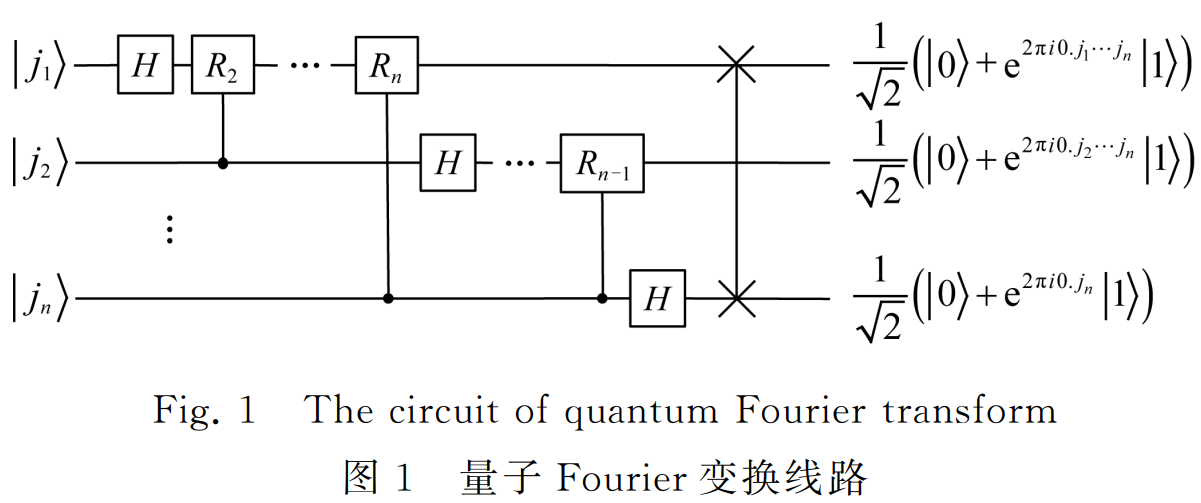
\includegraphics[width=0.90\textwidth]{img/ch2m1.png} 
\caption{量子 Fourier 变换线路}
\label{Test}
\end{figure}

通过量子 Fourier 变换可以实现相位估计,设 $|u\rangle$ 是酉算子 $U$ 的特征值为 $\mathrm{e}^{2 \pi i i q}$ 的一个本征态,则可大概率得到 $\varphi$ 的指定精度的近似值。相位估计是众多量子算法的关键部分,结合经典算法,可以有效解决求阶、求周期问题,更一般地可有效解决隐含子群问题。Deutsch-Jozsa 算法、 Shor 大整数分解算法、求离散对数等都是隐含子群问题的特例。目前大整数分解和求离散对数在经典计算机上还没有有效的求解方法,通过量子 Fourier 变换,在量子计算机上可有效求解,这也体现了量子计算较之经典计算的优越性。

\subsection{量子搜索}

量子搜索对无结构数据的搜索提供了二次加速。设在一个大小为 $N$ 的无结构数据空间中有 $M$ 个解,量子搜索通过大约 $\sqrt{N}$ 次操作,可以找到一个解。虽然没有基于量子 Fourier 算法的指数加速效果,但由于搜索问题的普遍性,量子搜索算法仍具有很大的意义。

\begin{figure}[htb]
\centering 
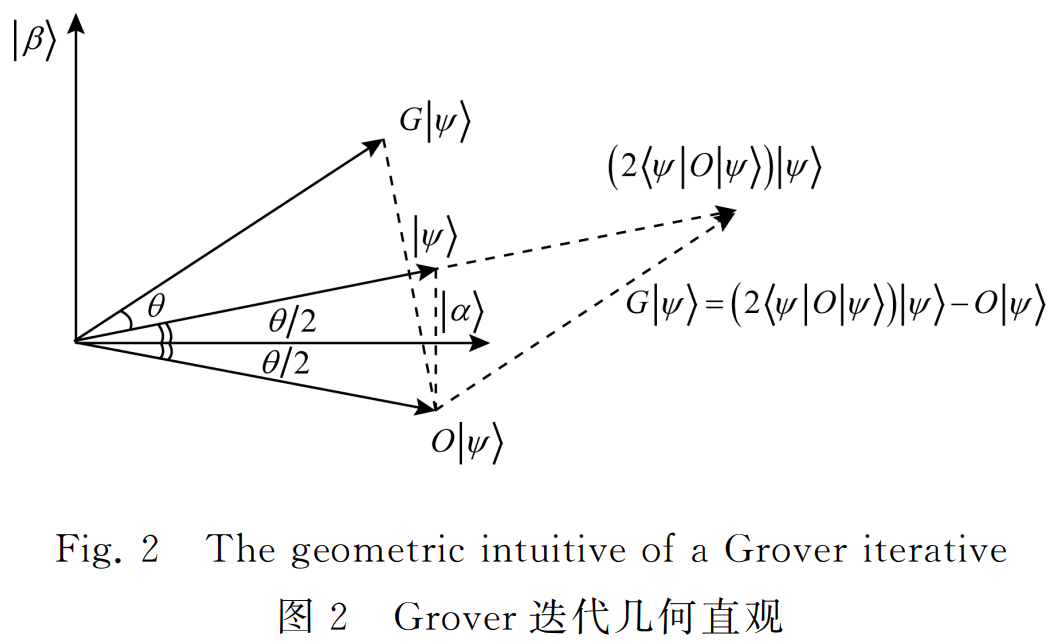
\includegraphics[width=0.90\textwidth]{img/ch2m2.png} 
\caption{Grover 迭代几何直观}
\label{Test}
\end{figure}

算法中使用了称为 Grover 迭代的算子,Grover 迭代可表示为 $(2|\psi\rangle\langle\psi|-I) O$ ,其中$|\psi\rangle=H^{\otimes n}|0\rangle$, $O$ 为识别搜索问题解的 Oracle。 直观上来看 Grover 迭代实现了由初始量子态和搜索问题解组成的均匀叠加态张成的二维空间中的一个旋转,如图所示。其中 $|\alpha\rangle=\sum_{x}|x\rangle \mid \sqrt{N-M}$ 为归一化的非搜索问题解的叠加态,$|\beta\rangle=\sum_{y}|y\rangle \mid \sqrt{M}$ 为归一化的搜索问题解的叠加态,$G$ 为 Grover 迭代算子,$\theta$ 满足 $\cos (\theta / 2)=\sqrt{(N-M) / N}$ 。每经过一次 Grover 迭代,初态 $|\psi\rangle$ 向 $|\beta\rangle$ 方向靠近 $\theta$。经过 $O(\sqrt{N})$ 次迭代, $|\psi\rangle$ 接近 $|\beta\rangle$,在计算基中测量将以很高的概率输出搜索问题的一个解。

\section{量子通信与量子密码研究进展}

BB84 协议提出后,量子密码学正式登上历史的舞台。量子密码学以量子密钥分发为核心,对应于经典密码学领域的其他研究分支也得到了广泛关注,并形成各个不同的研究分支。本文对量子密钥分发、量子加密、量子签名和其他研究领域这 4 个方面的主要思想及进展情况进行介绍。

\subsection{量子密码研究进展及主要思想}

\subsection{量子密钥分发}

密钥分发用来在通信双方 (Alice和 Bob) 安全分发一个密钥,后续可以用该密钥安全通信.BB84 协议是第一个量子密钥分发协议,被研究的最多,也最具代表性,在量子密码研究中占有重要地位,我们在此以 Bennett 和 Brassard 提出的原始协议为基础对其进行介绍。

BB84 协议使用光子作为量子态的载体,使用 2 组偏振基编码数据。一种为线偏振基並记为 $+$,水平偏振状态记为 $|\leftrightarrow\rangle$ ,垂直偏振状态记为 $|\updownarrow\rangle$,另一种为圆偏振基並记为 $\bigcirc$,左旋偏振状态记为 $|\nearrow\rangle$,右旋偏振状态记为 $|\searrow\rangle$。在这 2 组基下,比特“0”分别被编码为 $|\leftrightarrow\rangle$ 和 $|\nearrow\rangle$,比特“1”分别被编码为 $|\updownarrow\rangle$ 和  $|\searrow\rangle$ 。描述光子线偏振和圆偏振的力学量算符不可对易,由 Heisenberg 不确定性原理,这 2 种偏振状态无法被同时确定。BB84 协议需要一条量子信道和一条经典信道。其量子信道可以是光纤或自由空间,经典信道为普通的公共信道,安全性不需考虑。这 2 种信道都允许第三方 (Eve) 监听。

\begin{itemize}
\item [1.] Alice 对于某个安全参数 $n$,随机选择稍多于 $4n$ 个比特,对每个比特随机选取线偏振基或圆偏振基进行编码,并将编码后的光子序列通过量子信道发送给 Bob。
\item [2.] Bob 收到光子序列后,随机选取线偏振基和圆偏振基对光子序列进行测量。
\item [3.] Bob 与 Alice 通过经典信道联系,对比他们所选择的基序列,舍弃选择不同基的比特,一般而言,他们将得到稍多于 $2n$ 个比特。
\item [4.] Alice 选择 $n$ 个比特与 Bob 对比检查是否有第三方监听,如果错误率超过某一个阈值,则放弃本次协议其监听会造成对量子态的干扰,从而显着增大错误率。
\item [5.] Alice 和 Bob 对剩下的 $n$ 个比特执行密钥纠错和安全性增强,得到最终的密钥。
\end{itemize}

最后 BB84 协议的工作过程可用下图所示的例子直观描述。

\begin{figure}[htb]
\centering 
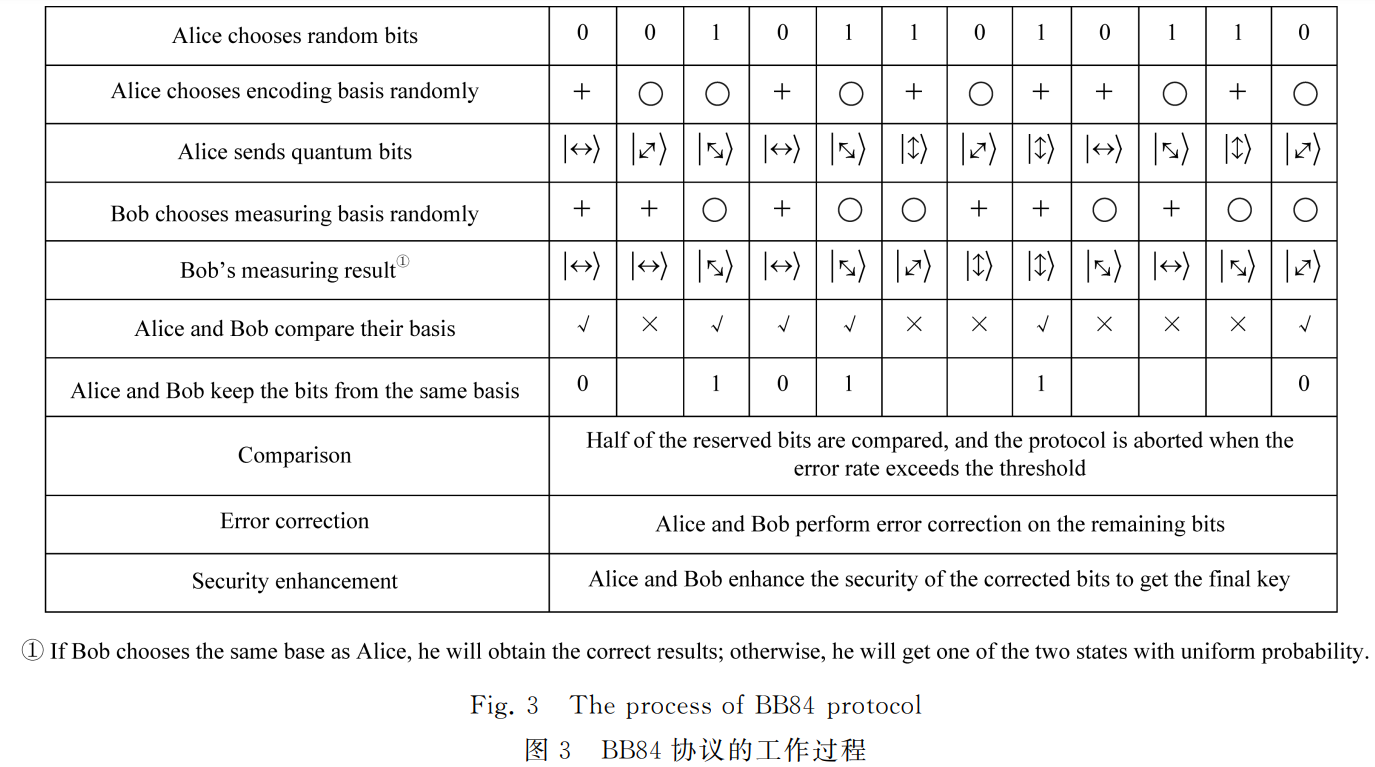
\includegraphics[width=0.90\textwidth]{img/ch2m3.png} 
\caption{BB84 协议的工作}
\label{Test}
\end{figure}
在 BB84 协议工作的过程中,Bob 收到 Alice 发送的光子序列后,并不知道 Alice 编码这些光子所用的基,他在随机选择测量基时,有 1/2 的概率和 Alice 使用的基相同,因此在作基比对后,他们能得到大概原始比特数一半的比特形成的序列,在这个比特序列中,由于设备、环境等因素的影响,会出现一定的错误,记错误率为 $\boldsymbol{\xi}_{0}$。如果协议过程中存在 Eve 监听, Eve 截获 Alice发送的光子序列后,受未知量子态不可克隆原理的限制,他无法对光子序列进行复制,为了获取信息,Eve 必须在原始光子序列上测量。然而, Eve 也不知道 Alice 编码光子所用的基,他只能随机选择测量基,在测量的过程中必然会
对光子产生扰动,使得在 Alice 和 Bob 作比特比对时,得到的错误率超过 $\boldsymbol{\xi}_{0}$,由此可以发现监听。

Alice 和 Bob 在比特比对后,需要对剩下的比特序列纠错,其基本思想是将这些比特序列分为若干区,对每个区进行奇偶校验,如果校验通过,则放弃一个比特后保留该区,如果校验不通过,则放弃整个区,经过若干次重复,可确保他们有非常高的概率持有相同的比特序列。纠错后 Alice 和 Bob 对共享比特序列进行安全性增强,如随机选择 Hash 函数对其进行压缩,得到最终的共享密钥。

不同于经典密码学的安全性基于数学困难问题, BB84 的安全性基于量子不可克隆和不确定性原理等物理学定律,它提供了无条件安全性, Shor 和 Preskill 于 2000 年对其进行了证明,确认了这是一个可证安全的密钥分配方案,符合现代密码学设计的基本要求。


\subsection{量子加密}

\subsubsection{量子一次一密}

1917 年 Vernam 提出了一种完善保密的加密方法,称为一次一密 (one-timepad).与之对应到量子密码学也有量子一次一密算法。根据明文、密钥和密文分别是经典比特还是量子比特,量子一次一密算法主要有 3 种类型。

\begin{itemize}
\item [1.] 使用 2 位经典比特加密一位量子比特明文,得到一位量子比特密文。该算法由 Boykin 和 Roychowdhury 提出。
\item [2.] 超密编码 : 由 Bennett和 Wiesner 首先提出。超密编码开始需要通信双方 Alice 和 Bob 共享一对处于纠缠态的量子比特,如 Bell 态.Alice 对自己手中的量子比特作 Pauli 门操作或不作任何操作后,将其发送给 Bob, Bob 通过对这一对纠缠比特作合适测量,可得到 Alice 想要发送的 2 位经典比特明文.超密编码可以看作是使用一位量子比特作为密钥,加密 2 位经典比特明文,得到一位量子比特密文。
\item [3.] 量子隐形传态 : 开始时 Alice 和 Bob 共享一个 EPR 对,每人拥有 EPR 对的一个量子比特。Alice 将待发送的量子态 $|\varphi\rangle$ 与自己手中的一半 EPR 对作联合测量,得到两比特的经典信息,然后其发给 Bob,Bob 可以根据这两比特信息对自己的一半 EPR 对作相应测量,得到 $|\varphi\rangle$ 。 Gisin 等人将其视为明文、密钥和密文都是量子比特的一次一密。
\end{itemize}

\subsubsection{量子公钥加密}

2000 年 Okamoto等人在美密会上首先提出了量子公钥加密方案。方案中消息的发送方、接收方以及敌手都被抽象成量子多项式时间图灵机,并且在量子计算模型下构造了量子单向陷门函数。在这之后,多种多样的量子公钥密码方案被提出。 2003 年 Yang 提出了一个基于经典 NP 完全问题的量子公钥加密方案。 2008 年 Nikolopoulos 基于量子比特旋转变换提出了一个公钥加密方案。2009 年 Gao 等人使用对称密钥构造了量子公钥加密方案。 2012 年 Liang 等人提出了一个信息论安全的加密方案。 2014 年 Zheng 等人提出了面向比特的概率型量子公钥加密方案。2015 年 Vlachou 等人提出了基于量子随机游走的方案。2017 年 Wu 等人提出了基于 Bell 态的公钥加密方案。

\subsubsection{量子同态加密}

2012 年 Rohde等人使用玻色子采样和量子行走模型实现了有限的量子同态加密。2015 年 Liang 基于通用量子线路,构造了量子全同态加密方案,该方案中可以对加密数据执行任意量子变换。 2015 美密会 上, Broadbent 和 Jeffery 基于经典 FHE 的存在提出了 2 种 QHE 方案。他们提供了 2 种不同的方法来完成具有有限数量的非 Clifford 门线路的同态加密,还提出了 QFHE 及其安全性的正式定义。 2016 年 Dulek 等人扩展了这项工作,以便有效地评估任意多项式大小的线路,并提供了一种新的紧凑型 QHE 方案。 2017 年 Ouyang 等人提出了一种 $(n,n)$ 阈值秘密共享方案,该方案允许对共享秘密上的量子线路进行评估而无需对其进行解码。此外还有一些其他的量子同态加密方案。

\subsection{量子签名}

量子签名是量子密码学的一个重要分支,在 2001 年由 Gottesman 等人首次提出,它通过量子力学原理保证数据签名的安全性。同经典签名一样,其安全性需要满足 3 个属性。

\begin{itemize}
\item [1] 不可伪造,没有人能伪造一个合法的签名。
\item [2] 不可否认,签名者不能对自己的签名否认。
\item [3] 可公开验证,接收到消息的任何人均可通过。
\end{itemize}

公钥验证消息签名的合法性,人们最开始研究的量子签名是依赖于仲裁的,第一个具体方案由 Zeng等人在 2002 年提出,此后 Curty 等人、Zou 等人、Gao 等人利用经典签名协议的分析方法,给出了该方案的一些安全漏洞。2009 年 Li 等人提出了基于 Bell 态的仲裁量子签名。2015 年 Li 和 Shi 提出了基于 CNOT 链加密的仲裁量子签名。2018 年 Feng 等人提出了基于连续变量量子态的仲裁量子签名。

\section{密码学界面对威胁的应对}


面对量子计算突飞猛进的威胁,密码学界以美国国家标准与技术研究院 (NIST) 为首,早早就开始了应对布局,全面开展了一种公开的程序挑选一个或多个公钥密码算法的进程。这些新的公钥密码标准将为数字签名、公钥密码以及密钥建立算法规定一个或多个另外的算法。新标准将对 FIPS 186-4 数字签名标准 (DSS) 以及特别出版物 800-56A 版本 3 (使用离散对数密码的双序密钥建立方案建议) 和 SP 800-56B (使用整数因子分解的双序密钥建立方案建议) 进行扩充。 NIST 的意图是,在可以预见的未来,包括量子计算机出现之后,这些算法将能够保护美国政府的敏感信息,这个竞赛过程称为 NIST PQC 后量子密码标准化进程。

PQC 标准化进程是 NIST 对量子计算机技术发展的响应。量子计算机利用了量子力学现象来求解困难的或传统计算机难以处理的难题。如果大容量规模的量子计算机被建造出来了,它们将能够破解 NIST 目前标准化的这些公钥密码系统,包括数字签名和密钥建立方案。量子计算机对对称密码系统也有一定的影响,但其影响并不强烈。后量子密码的目标,是发展对量子计算机和经典计算机都安全的密码系统,并且能够与现有协议和网络互操作。在启动 PQC 标准化进程之前, NIST 于 2015 年 4 月就成立了一个工作组,讨论与后量子密码以及未来可能的标准化相关的问题。一年之后,NIST 发布了后量子密码报告 NISTIR,共享了 NIST 对量子计算和后量子密码的状态的理解,概括了 NIST 推进该领域的初始计划, NIST 于 PQCrypto 2016 会议上以报告形式宣布了 PQC 标准化进程的初步细节。

2016 年 8 月,NIST 以一个联邦注册公告的方式,公布了对后量子密码的公开注释建议的要求和评估判断准则。此后,又基于公开的反馈意见,对这些要求和评估判断准则进行了更新,并且稍后将它们包含在 2016年 12 月 20 日的第二次联邦注册公告 FRN-Dec16 内。该公告正式征集关于后量子密码算法的公开提案,标志着 NIST 开始了 PQC 标准化的进程。候选提案的最后期限预定在 2017 年 11 月 30 日,在那个时日,NIST 接收到了 82 个提案包。这是世界范围内密码社区,在1998年为高级加密标准竞赛提出过21个候选算法,在2008年为安全哈希算法3 (SHA-3)竞赛提交过 64 个文件包作出的强烈反应, NIST 于 2017 年 12 月20 日宣布接受了满足提交要求和最小接受判断准则的 69 个第一轮候选算法。这 69 个提案包含了 20 个数字签名方案和49个公钥密码 (PKE) 或密钥封装机制 (KEM)。第一轮候选算法的提交包都被在线张贴在https://www.nist.gov/pqcrypto 网页上,征求公开的评论和注释。

NIST 于 2018 年 4 月11-13 日在佛罗里达 Lauderdale 组织了第一次 PQC 标准化会议,其研究成果收录在 PQCrypto 2018中。获得接受的第一轮候选算法的提交者被邀请到会上介绍他们的算法。NIST 还讨论了其缩小候选算法池、聚焦整个社区的关注点以及启动第二轮标准化进程的计划。在第一轮竞赛中,NIST接收到密码社区的大量反馈。基于对第一轮候选算法的公开反馈和内部评估,NIST 于 2019 年 1 月 30 日宣布挑选出 26 个算法作为第二轮候选算法,进入该标准化进程的第二阶段。2019 年 7 月 20 日宣布挑选出其中的7个算法作为第三轮最终候选算法 PK,另外 8 个算法作为后补。

最终入选 7 算法如下:

\subsection{CRYSTALS-KYBER}


Kyber 为一簇密钥封装机制,它基于模误差学习(MLWE) 问题的后量子困难问题假设,提供选择性的密文安全性(即IND-CCA)。Kyber 包含了一个标准的带误差学习 (LWE) 风格的 CPA 安全的公钥密码方案,其基础的代数目标是在 2 的幂次的圆分割环上的一个模。通过对这个参数的精选,使其能够采用数论变换 (NTT) 进行效率非常高的计算。其噪声按照一个有中心的二项式分布来进行采样。CCA 安全性是通过 Fujisaki-Okamoto 变换的一种著名的变体来达到,其中会话密钥是基于一种加密的方法来传送的。对 Kyber 的安全性强度水平的调整十分简单。一种调整是仅仅改变底层模的秩序(在{2,3,4}的范围内),并且调整其噪声分布参数(分别在{5,4,3}的范围内)。对于密钥交换而言,Kyber 的性能为最具竞争力的密钥交换设计之一。

Kyber 的安全性依赖于一个已深入研究问题的变体。其提交文档提供了一种基于随机预言模型 (ROM) 的严密安全性证明,以及一种基于量子随机预言模型 (QROM) 的非严密安全性证明,二者都是基于 MLWE 假设。我们注意到一个潜在的问题是,这个安全性证明并不直接应用于 Kyber 自身,而是应用于该方案的一个不压缩公钥的改进版本。如果没有这种改进,Kyber 实际上是依赖于一个不同的(或附加的)类似取整的假设。如果是这样的话,将带来密码分析上的担忧,因为在MLWE和模取整学习(MLWR)之间进行的那些已知的缩减设计,可能并不要求Kyber选取的那些参数。

\subsection{NTRUEncrypt 与 NTRU-HRSS-KEM 合并的 NTRU}

NTRU密码为一种基于格的单向 CPA 安全(OW-CPA)的公钥密码方案,它大约发明于 1996年。经过了数十年的研究,NTRU 密码的安全性已经得到了相当好的理解和深入的研究审查。已经发展出该方案的许多变体及其派生出的密钥封装机制,包括 NTRUEncrypt 和 NTRU-HRSS-KEM 方案。这两个提案已经宣布合并为一种方案,称之为 NTRU。NTRU 的安全性基础是比 LWE 或 RLWE 稍微强一点的一种假设,有时称之为 NTRU 假设。在这个合并中, KEM 为一种严密的 IND-CCA2 安全性转换,源自于量子随机预言模型的一种确定性 OW-CPA 安全的公钥密码方案。该提案对于 KEM 中的确定性PKE具有两个选项。其派生的 KEM 没有解密失败问题,同时避免了密钥产生期间的“对1值的评估”和可逆校验这两个问题。该方案以三个环结构实例详细说明了三个参数集。KEM 产生的密钥和密文都具有良好的尺寸,其封装和解封效率看起来都很高。虽然它没有形成已知的安全薄弱点,在具有相似效率的 RLWE 和 MLWE 密码系统中,NTRU的构造产生的结构稍多一些(由于其矢量比期望的矢量更短)。这个方面还需要进一步研究。

\subsection{SABER}

SABER 是一个基于格的 PKE 和 KEM 簇,它基于取整的模学习量子困难问题来达到 CPA 和 CCA 安全性。该方案使用在一个2的幂次的分圆环上具有固定维度和模数的不同秩的多个模块,其安全级别分别为 1、3 以及5。其 MLWR 秘密分布为有中心的二项式分布,其会话密钥哈希值再由公钥进行哈希运算,以实现多目标防护。其多项式相乘按照 Toom-Cook 和 Karatsuba 的详细描述进行。该方案通过 Fujisaki-Okamoto 变换的一个变量来达到 CCA 安全性。其会话密钥使用一种基于带噪声的密钥一致性协调的密码方法来传送。在所有后量子密钥交换中,SABER的性能优势具有非常强的竞争力。在每个安全级别中,它的带宽代价都是比较低的。关于 SABER 安全性的最明显担忧,是它是否过分扩展了(模)取整学习的实际难度。虽然尚未有已知的利用所选参数的与 (M)LWR 相关的攻击,在取整样本 MLWE 和 MLWR 之间仍然存在很宽泛的缩减空间,并且还没有应用到 SABER 中。NIST 将 SABER 当作一个机遇,以突出对具有较小参数和取整样本的 (M)LWR 进行深入分析的需求,有利于推进该方面的研究工作,继续全面增强对该假设的信心。

\subsection{Classic McEliece}

Classic McEliece 是一种 IND-CCA2 安全级别的密钥封装机制 (KEM)。该提案以有名的 McEliece 密码系统为基础,McEliece 密码系统为 1978 年公布的第一个基于编码的公钥密码系统。该 KEM 的公钥机制确定一个随机二元 Goppa 码,通过在码字上加入误差来产生密文,通过解码来实现解封。其安全性基于解码一个常规线性码的难度,并且假设一个随机二元 Goppa 码不能通过一个随机线性码来辨别。其安全问题已经具有很长的分析研究历史,但并没有显著改变其攻击复杂度。 Classic McEliece 也具有产生的密文非常短的特点,大概 200 个字节左右,看起来具有良好的封装和解封性能。McEliece 类型的密码系统的主要缺点是具有很大的公钥尺寸,超过了一百万个字节。该提案仅仅包含了第5类安全性的参数集,因而希望提交者生成其它安全类别的参数集。

\subsection{CRYSTALS-DILITHIUM}

Dilithium 为一种格基签名方案,采用了Fiat-Shamir启发方法来构造,其安全性是依赖于MLWE的困难问题。Dilithium 与密钥交换机制 Kyber 都是 CRYSTALS 的组成部分。Dilithium 的主要新颖性在于通过忽略一些低阶 bit 来减小其公钥尺寸;为了进行补偿,每个签名都包含了一个额外的“线索”,允许验证者对签名进行核对。Dilithium 提供了相当良好的性能,其实现也相对简单。对 Dilithium 的最知名的攻击是基于格的偏移缩减,这种攻击没有有效利用MLWE问题的代数结构。Dilithium 的参数选择以对这些攻击代价的保守估计为基础。Dilithium 具有一个基于经典随机预言机模型的形式化的安全性证明。这个证明是极不平凡的,它突破了量子随机预言机模型;但是还没有任何已知攻击的实例。NIST 鼓励对这个方案的所有方面都进行深入的分析研究。

\subsection{FALCON}

FAlCON 为一种格基签名方案,它基于 GPV(Gentry-Peikert-Vaikuntanathan) 高斯取样,应用了NTRU格。其主要的创新性在于,它应用了一种树形的数据结构(即 FAlCON 树),使其成为对高斯采样的一种非常快的递归算法。对 FAlCON 方案的最知名的攻击是基于格的偏移缩减,这种攻击没有有效利用 NTRU 格的特殊结构。FAlCON 具有一个基于经典随机预言机模型的形式化的安全性证明。FAlCON 提供了非常优良的性能,但是其实现相当复杂,因为它严重依赖于数域的多域塔结构,并且需要双精度浮点算法。该方案还需要进行更多的研究工作,确保其签名算法面对边信道攻击时是安全的。

\subsection{Rainbow}

Rainbow 是一种多变量数字签名方案,它是 UOV 结构的一种推广,允许进行参数优化,使其以增加代数结构的代价获得更高的效率。Rainbow 签名方案所提交的格式已经具有长达 15 年的针对各种参数的研究历程。Rainbow 方案声称,由于使用了随机加盐的一种哈希构造,因而具备 EUF-CMA 安全性。Rainbow 参数谱允许在各种各样的大量应用场景中进行优化。Rainbow 的另一优势是它已经在其它包括轻量级应用在内的场景中得到了研究。Rainbow 提案针对 NIST 号召建议中的所有安全级别,提供了若干个参数集。作为一种入选第二轮的候选算法,期望能够将研究重点聚焦于一组更窄的细节规格上面。此外,还希望能激发针对 Rainbow 密钥以及文献中已有的、而 Rainbow 提案中并未考虑的那些优化技术开展更多的研究,最终使研究社区在方案的可行性上面取得一致。此外,Rainbow 的实现也可能得到很大的改进。

实际上我们并不处在建造一台有能力破译目前公钥密码(学)的量子计算机的中期阶段(例如5年)内。执行肖尔算法所需的量子比特的数量,远远超过今天我们制造的最强大的量子计算机的能力,而且肖尔算法大规模的可靠的应用还没有被展示出来。今天,我们并不清楚诸如量子比特的退相干和管理噪声以减少量子系统中的差错等面临的挑战能否被解决。正因为如此,在短期或者中期内建造这样一台可规模化的扩展的量子计算机似乎不太现实。

然而,放眼较长的时间(20年),忽视量子计算机对于目前的现代密码学标准的威胁将会是错误的。正如美国国家标准与技术研究院的描述:“一些人预测在接下来的20年左右,足够规模的量子计算机会被制造出来,基本上可以打破目前使用中的所有公钥方案。在历史上,我们花了差不多20年时间去配置现代公钥密码基础架构。因此,不论我们能否准确估计量子计算时代到来的时间,我们都必须现在开始准备我们的信息安全系统,使之能够对抗量子计算”。

%\begin{figure}[htb]
%\centering 
%\includegraphics[width=0.90\textwidth]{img/XXX.png} 
%\caption{官网}
%\label{Test}
%\end{figure}
